\documentclass[tikz]{standalone}
\usepackage{pgfplots}
\pgfplotsset{compat=1.15}
\usepackage{mathrsfs}
\usetikzlibrary{arrows,calc}
\usepackage{tkz-euclide}

\pagestyle{empty}

\definecolor{AngleClr}{rgb}{0,0.39215686274509803,0}
\definecolor{ShapeClr}{rgb}{0.6,0.2,0}

\begin{document}

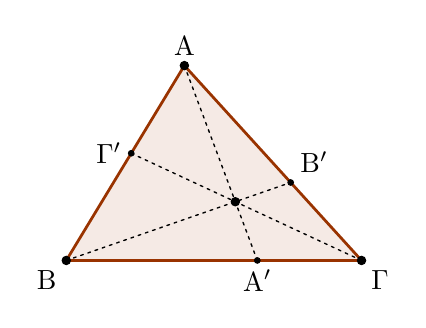
\begin{tikzpicture}[scale=.75]
\tkzSetUpLine[line width=1pt,color=black]
\tkzSetUpPoint[fill=black]

\tkzDefPoints{0/0/B,2/3.3/A,5/0/C}

\tkzDefTriangleCenter[in](A,B,C)
\tkzGetPoint{I}

\tkzDefPointOnLine[pos=0.45](A,B)\tkzGetPoint{CC}
\tkzDefPointOnLine[pos=0.6](A,C)\tkzGetPoint{BB}

\tkzInterLL(B,BB)(C,CC) \tkzGetPoint{I}
\tkzInterLL(A,I)(B,C) \tkzGetPoint{AA}

\tkzFillPolygon[fill=ShapeClr,fill opacity=0.1](A,B,C)


\tkzDrawPolygon[color=ShapeClr](A,B,C)

\tkzDrawSegments[line width=0.5pt,color=black,dashed,dash pattern=on 1pt off 1.75pt](A,AA B,BB C,CC)


\tkzDrawPoints[size=3](A,B,C,I)
\tkzDrawPoints[size=2](AA,BB,CC)
\tkzLabelPoint[above](A){$\rm A$}
\tkzLabelPoint[below left](B){$\rm B$}
\tkzLabelPoint[below right](C){$\rm \Gamma$}
\tkzLabelPoint[below](AA){$\rm A'$}
\tkzLabelPoint[above right](BB){$\rm B'$}
\tkzLabelPoint[left](CC){$\rm\Gamma'$}


\end{tikzpicture}

\end{document}
